Degree of freedom (DOF) is the number of independent parameters that can be varied in a mechanical system.
Simply put the DOF of a robot is the number independent joints the robot contains.
In modern robot implementation each joint is controlled by an actuator.
Each actuator is controlled by the controller.
The more DOF the more complex the controller.

In the early 1930s simple two DOF robots were used by the soviets as explosive devices\cite{robotTelitankSpringer2013military}.
These robots were remote control and had no mind of their own.
In 1948 William Grey Walter created the first autonomous robots \textit{Tortoise Elmer} and \textit{Elise}\cite{robotElmer}.
Each of these simple two DOF robots were programmed in hardware to go towards a light source.  
This was referred to as BEAM Robot (Biology, Electronics, Aesthetics, and Mechanics) because of how the hardware configuration mimicked the electrical connections in an animals brain.
In later years robots were being programmed in software to help create the first industrial robot UNIMATE which was a 6 DOF arm created by General Motors in 1954\cite{handbookOnRobotics2008springer}.  
Lunokhod 2, a soviet lunar rover which landed on the moon in 1973, was equipped with a laser ranging system and a TV camera.
It contained 11 DOF and had automated systems onboard, however it was primarily a remote controlled vehicle.
By 1986 Rodney Brooks, co-founder and CTO of iRobot Corp., created Allen, a 18 DOF humanoid robot.
The complexity and number of DOF keeps on increasing.
By 1997 Honda completed the 28 DOF P3, a early version of what will become ASIMO \cite{robotsAsimo1041641}.
Today with the presents of HUBO, ASMO and HRP-4C it is common place for a robot to contain upwards of 40 DOF.
A study done on 180 robots from the early 20$^{th}$ century to the present projects that by the year 2020 it will be as common to have a 70 DOF robot as it is to have a 40 DOF robot in 2013, see Fig.~\ref{fig:numOfRobots}. 
\textit{The trend of increasing DOF in robots makes creating a control structure for these systems timely.}


These high DOF robots require complex control systems and strategies.



Creating controllers for these high degree of freedom complex systems is essential for development of the next generation of robots.
Due to the inherent complexity and often high expense of these systems, controllers must be able to be tested and verified.



\begin{figure}[thpb]
  \centering
      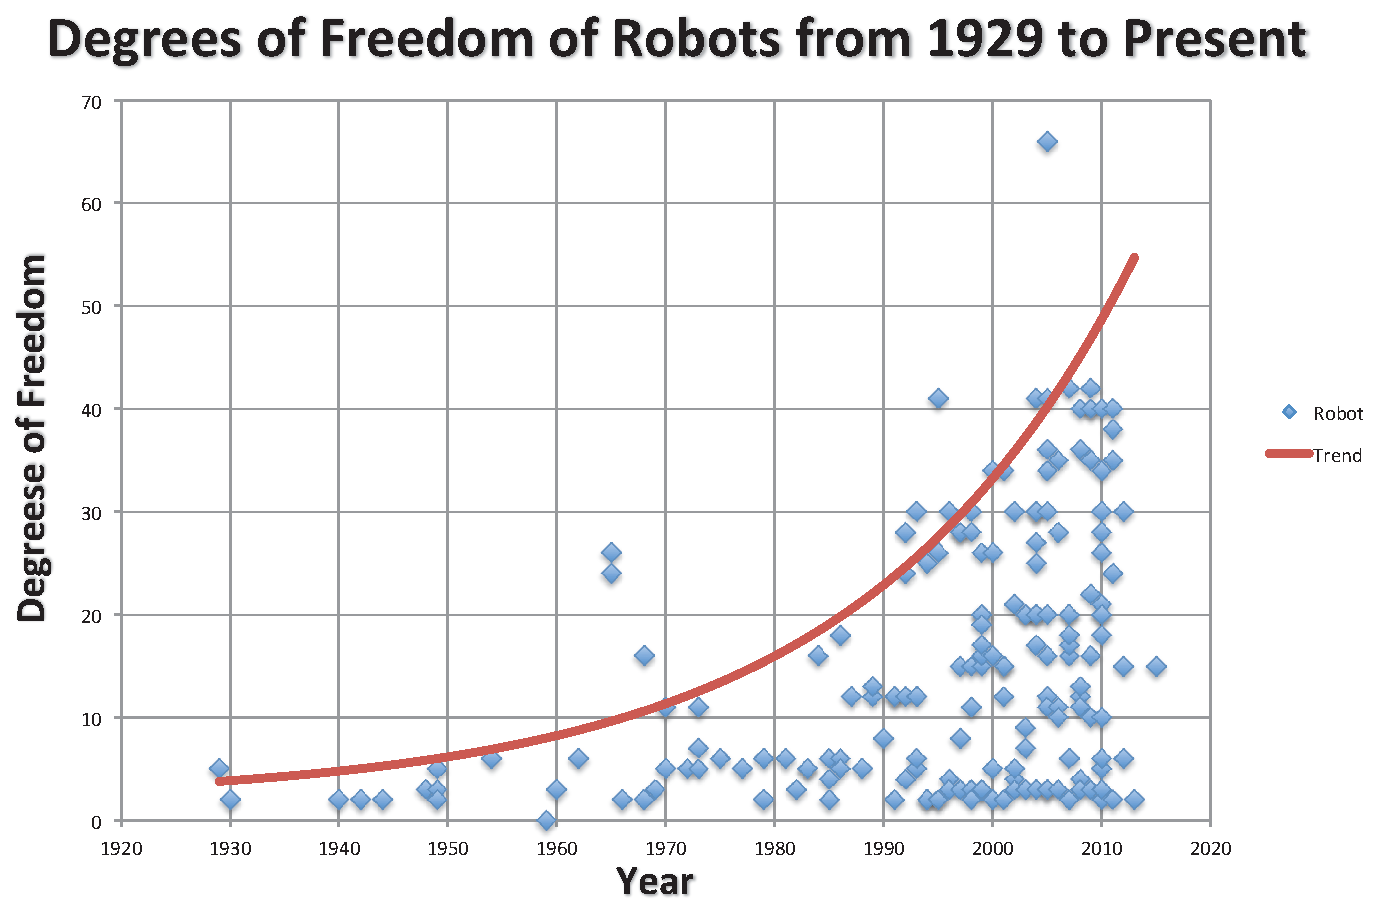
\includegraphics[width=0.8\columnwidth]{./pix/robotsDOF.pdf}
\caption{Number of degrees of freedom for robots form 1929 to the present.}
\label{fig:numOfRobots}
\end{figure}

